\documentclass[11pt,a4paper]{article}
\usepackage[margin=2.3cm]{geometry}
\usepackage[T1]{fontenc}
\usepackage[utf8]{inputenc}
\usepackage{amsmath,amssymb,lmodern,microtype,booktabs,longtable,array,xcolor,enumitem,tikz,pgfplots,tcolorbox,fancyhdr,titlesec,graphicx,float}
\usepackage[hidelinks]{hyperref}
\pgfplotsset{compat=1.16}
\usetikzlibrary{arrows.meta,positioning,shapes.geometric,calc}
\definecolor{acc}{HTML}{1F4E79}\definecolor{ok}{HTML}{2E7D32}\definecolor{warn}{HTML}{B26A00}\definecolor{bad}{HTML}{B3261E}
\titleformat{\section}{\Large\bfseries\color{acc}}{\thesection}{0.6em}{}
\titleformat{\subsection}{\large\bfseries\color{acc}}{\thesubsection}{0.5em}{}
\setlist{itemsep=2pt,topsep=3pt}
\pagestyle{fancy}\fancyhf{}\fancyfoot[C]{\thepage}\fancyhead[L]{\small HL-LHC idea discovery}\fancyhead[R]{\small Progress report, 6 Oct 2026}
\renewcommand{\arraystretch}{1.15}
\newtcolorbox{key}[1][]{colback=acc!6,colframe=acc,boxrule=0.6pt,arc=2pt,left=6pt,right=6pt,top=4pt,bottom=4pt,#1}
\newtcolorbox{caution}[1][]{colback=warn!8,colframe=warn,boxrule=0.6pt,arc=2pt,left=6pt,right=6pt,top=4pt,bottom=4pt,#1}
\begin{document}
\begin{titlepage}
\centering\vspace*{2.5cm}
{\Huge\bfseries\color{acc} Discovering under-explored HL-LHC\\[4pt] phenomenology ideas}\\[1.2cm]
{\Large Autonomous multi-agent literature review: method, results and lessons}\\[1.5cm]
{\large Progress report on the discovery phase}\\[0.6cm]
{\large 6 October 2026}\\[2cm]
\begin{minipage}{0.8\textwidth}\small
Workspace: \texttt{hllhc\_search/} (local project; nothing installed globally).\\
Orchestrator: Claude Sonnet 5.5 in Claude Code. Sub-agents: Sonnet 5.5, Opus 5.5 and the strongest available model (``fable'') as arbiter.\\
Status: discovery phase complete, \textbf{waiting for the human choice of direction}. Stage~2 (analysis design) has not started.
\end{minipage}
\vfill
\end{titlepage}
\tableofcontents\newpage

\section{Executive summary}
\begin{key}
\textbf{Question.} Which established theoretical ideas have experimental consequences that CMS/ATLAS have not fully covered, and could plausibly become a useful HL-LHC analysis?\\[3pt]
\textbf{Answer so far.} After an extensive search, \textbf{no candidate survived intact}. For all ten directions that received full independent review, a phenomenology paper already proposes the analysis; what remains open is the \emph{experimental execution} (an ATLAS/CMS analysis, a recast, or a collaboration-level HL-LHC projection), not a new theoretical idea. Several of the scouts' most attractive gaps were overturned by independent checks.
\end{key}

\begin{itemize}
\item \textbf{Corpus:} 986 unique papers (1975--2026), 483 PDFs downloaded and converted to text, 5,711 cached INSPIRE responses, 1,318 logged scout queries.
\item \textbf{Funnel:} 199 raw seeds $\to$ 74 merged directions $\to$ Gate~2: 27 PASS / 37 HOLD / 10 REJECT $\to$ Gate~3 adversarial on 27: 26 narrowed, 1 died, 0 intact $\to$ 10 fully reviewed $\to$ arbiter ranking: 2 tier~A, 5 tier~B, 3 tier~C (Section~\ref{sec:ranking}).
\item \textbf{Agents:} 55 sub-agent launches (16 Sonnet, 38 Opus, 1 arbiter on the strongest model); 20 Opus launches were interrupted by session rate limits and partly rerun.
\item \textbf{Top of the ranking:} C001 quirks (tier~A), C005 Higgs-portal dark showers in the tracker (tier~A), then C019, C044, C015, C051, C003 (tier~B), and C008, C040, C066 (tier~C).
\item \textbf{All 204 cited reference IDs in the final documents resolved on INSPIRE;} two numbers are flagged \textsc{unverified}.
\end{itemize}
\begin{caution}\textbf{Main caveat.} Only 10 of 74 directions got the full review (lean budget chosen by the user). Triage was done by Sonnet with abstract-level coverage checks, so parked directions may include missed opportunities and some rejections could be wrong; every rejection names its covering result so it can be checked.\end{caution}

\section{Objective and method}
The brief asked for a deep, citation-driven literature review, not an analysis. The design follows the MIT/JFC philosophy \emph{phase $\to$ written artifact $\to$ independent review $\to$ correction $\to$ next phase}: an orchestrator that does not do the reading itself, specialised sub-agents, mutually blind reviewers, and a human decision point at the end. Adaptations to the original brief are listed below.
\begin{itemize}
\item Added an \emph{archaeology} scout for old/orphaned ideas and two extra clusters (QCD/substructure, quantum-information observables).
\item Reviewers (experimental, feasibility, theory, adversarial) see only a neutral candidate description, never each other's conclusions.
\item Every cited reference ID is checked against INSPIRE (citation audit).
\item Cost cap: the plan required approval before exceeding about 40 strong-model runs; the user selected a ``lean'' budget (about 25 runs).
\end{itemize}
\subsection{Pipeline}
\begin{center}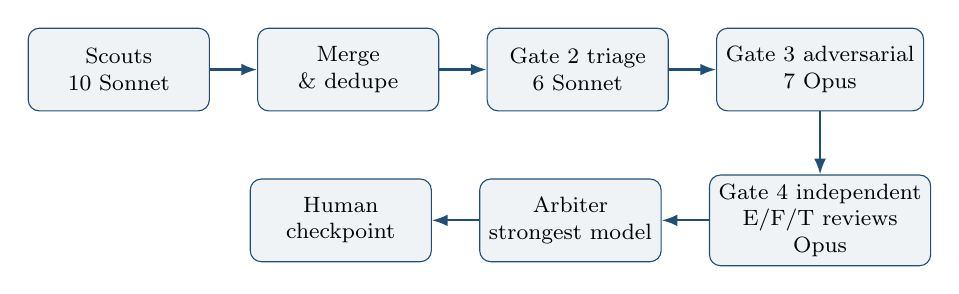
\begin{tikzpicture}[node distance=6mm,box/.style={draw=acc,fill=acc!7,rounded corners,align=center,minimum width=2.3cm,minimum height=1.05cm,font=\footnotesize},arr/.style={-{Latex[length=2mm]},thick,acc}]
\node[box](a){Scouts\\10 Sonnet};\node[box,right=of a](b){Merge\\\& dedupe};\node[box,right=of b](c){Gate 2 triage\\6 Sonnet};\node[box,right=of c](d){Gate 3 adversarial\\7 Opus};
\node[box,below=8mm of d](e){Gate 4 independent\\E/F/T reviews\\Opus};\node[box,left=of e](f){Arbiter\\strongest model};\node[box,left=of f](g){Human\\checkpoint};
\draw[arr](a)--(b);\draw[arr](b)--(c);\draw[arr](c)--(d);\draw[arr](d)--(e);\draw[arr](e)--(f);\draw[arr](f)--(g);
\end{tikzpicture}\end{center}
\subsection{Environment and tools}
Verified at the start (not assumed): INSPIRE REST API, arXiv API and PDF download, HEPData, WebSearch/WebFetch, Python~3.14 with the standard library only, \texttt{pdftotext}, \texttt{jq}. No MCP research server was relevant. Custom tools written in \texttt{research/tools/}: \texttt{inspire.py} (search, references, citations; cached, rate limited), \texttt{arxiv\_pdf.py} (download, convert, extract ``future work''-type sentences), \texttt{merge\_seeds.py}, and the generators for this report.
\subsection{Search strategy}
\begin{enumerate}
\item \textbf{Seminal discovery:} INSPIRE top-cited queries per cluster, including date $<$ 2012 to reach older ideas; reviews and white papers (Snowmass, HL/HE-LHC Yellow Report).
\item \textbf{Citation chains:} \texttt{refersto:recid} and \texttt{citedby:recid} to follow descendants and ancestors; each ``future work'' lead was checked by forward citations.
\item \textbf{Gap-phrase mining:} phrases such as ``unexplored'', ``blind spot'', ``dedicated search'' combined with cluster terms, then verbatim sentences extracted from PDFs. Treated as leads, never as evidence.
\item \textbf{Experiment-side mapping:} collaboration-filtered INSPIRE searches, public result pages, HEPData, recasts and Phase-2 projection documents.
\end{enumerate}

\section{Literature covered}
The scouts collected \textbf{986 unique papers} spanning 1975--2026. These were harvested as INSPIRE records (title, authors, abstract, citation count); 483 full-text PDFs were downloaded and converted, mostly to extract gap sentences and to let reviewers read the closest experimental results. \textit{Read} therefore means different things at different stages: \emph{metadata and abstract} for the bulk, \emph{full text} for the subset below.
\begin{caution}The exact number of papers read in depth is not tracked per agent. A fair statement is: all 986 were seen at metadata/abstract level; 483 PDFs were converted to text; the final dossiers rest on full reading of a few hundred sources, concentrated on the closest 3--5 experimental results and the source papers of the ten reviewed candidates.\end{caution}
\subsection{Papers by role and by decade}
\begin{center}\begin{tabular}{lr}\toprule Role (scout judgement) & Papers\\\midrule
Seminal / idea-introducing & 204\\
Phenomenology follow-ups & 326\\
Experimental searches / measurements & 336\\
Reviews / white papers & 80\\
HL-LHC / future projections & 30\\
Recasts / reinterpretations & 10\\
\midrule Total & 986\\\bottomrule\end{tabular}\end{center}
\begin{center}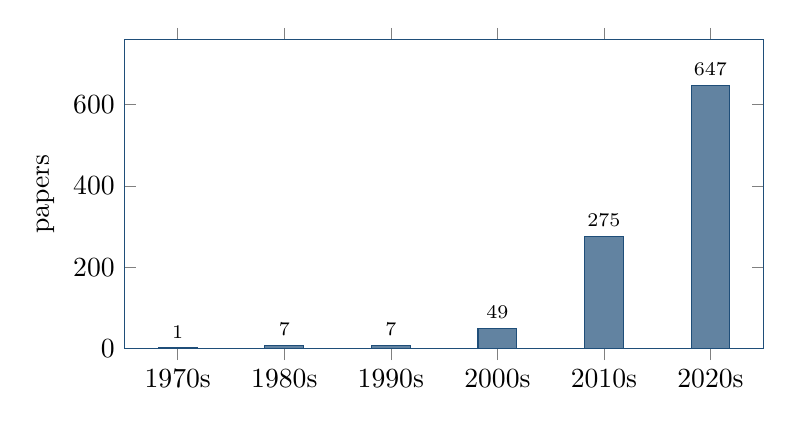
\begin{tikzpicture}\begin{axis}[ybar,width=0.8\textwidth,height=5.5cm,bar width=14pt,symbolic x coords={1970s,1980s,1990s,2000s,2010s,2020s},xtick=data,ylabel={papers},nodes near coords,every node near coord/.append style={font=\scriptsize},ymin=0,ymax=760,fill=acc,draw=acc]
\addplot[fill=acc!70] coordinates {(1970s,1) (1980s,7) (1990s,7) (2000s,49) (2010s,275) (2020s,647)};\end{axis}\end{tikzpicture}\\[-2pt]{\small Publication decade of the collected corpus. The weight on 2020s reflects the search for current experimental coverage; older ideas are the 1975--2009 tail.}\end{center}
\subsection{Per-cluster yield}
\begin{center}\small\begin{tabular}{lrr}\toprule Cluster & Papers (first tag) & Candidate seeds\\\midrule
ALPs \& light states & 104 & 18\\
Compositeness \& heavy states & 112 & 16\\
Dark sectors \& portals & 139 & 19\\
EFT \& EW precision & 117 & 18\\
Exotic Higgs \& scalars & 105 & 19\\
Leptoquarks \& flavour & 93 & 19\\
Long-lived particles & 66 & 21\\
Older / orphaned ideas & 69 & 26\\
QCD, substructure, quantum info & 93 & 22\\
SUSY corners & 88 & 21\\
\midrule Total & 986 & 199\\\bottomrule\end{tabular}\end{center}
\section{Seminal papers found}\label{sec:seminal}
The scouts tagged 204 papers as seminal and 80 as review. The tags are scout judgements, not a verified ranking. Each table lists the most-cited seminal papers per cluster; the full list is in \texttt{research/literature/seminal\_papers.md}.
\begin{key}\textbf{Which seminal ideas became research programs?} The best match to the ``latent research program'' pattern is the \emph{hidden-valley family}: Strassler--Zurek (hep-ph/0604261, 2006) $\to$ emerging jets $\to$ dark-shower benchmarks $\to$ SUEP $\to$ semi-visible jets, with experiments covering prompt and part of the displaced regimes only. The oldest lineages are quirks (Kang--Luty, 0805.4642) and the doubly charged Higgs (INSPIRE:214561, 1985). No forgotten idea was found whose collider consequence had \emph{never} been revisited: in every case a later paper or search had followed it up.\end{key}
\subsection*{ALPs \& light states}
\begin{center}\footnotesize\begin{tabular}{@{}p{2.5cm}rr p{9cm}@{}}\toprule ID & Year & Cites & Title\\\midrule
1708.00443 & 2017 & 694 & Collider Probes of Axion-Like Particles\\
1403.1269 & 2014 & 524 & Quark flavor transitions in Lmu-Ltau models\\
1509.00476 & 2015 & 382 & Probing MeV to 90 GeV axion-like particles with LEP and LHC\\
1701.05379 & 2017 & 348 & ALPs Effective Field Theory and Collider Signatures\\
1607.06083 & 2016 & 339 & Searching for Axionlike Particles with Ultraperipheral Heavy-Ion Collisions\\
2110.10698 & 2021 & 306 & Flavor probes of axion-like particles\\
\bottomrule\end{tabular}\end{center}
\subsection*{Compositeness \& heavy states}
\begin{center}\footnotesize\begin{tabular}{@{}p{2.5cm}rr p{9cm}@{}}\toprule ID & Year & Cites & Title\\\midrule
INSPIRE:99112 & 1975 & 2614 & Exact Left-Right Symmetry and Spontaneous Violation of Parity\\
hep-ph/0412089 & 2004 & 1809 & The Minimal composite Higgs model\\
INSPIRE:159286 & 1980 & 1238 & Technicolor\\
hep-ph/0604261 & 2006 & 1093 & Echoes of a hidden valley at hadron colliders\\
hep-ph/0502182 & 2005 & 975 & Little Higgs review\\
hep-ph/9411426 & 1994 & 969 & Topcolor assisted technicolor\\
\bottomrule\end{tabular}\end{center}
\subsection*{Dark sectors \& portals}
\begin{center}\footnotesize\begin{tabular}{@{}p{2.5cm}rr p{9cm}@{}}\toprule ID & Year & Cites & Title\\\midrule
hep-ph/0101138 & 2001 & 1128 & Inelastic dark matter\\
hep-ph/0605188 & 2006 & 988 & Higgs-field portal into hidden sectors\\
1402.5143 & 2014 & 730 & Mechanism for Thermal Relic Dark Matter of Strongly Interacting Massive Particles\\
hep-ph/0001179 & 2000 & 595 & Updated bounds on millicharged particles\\
0906.5614 & 2009 & 579 & Exploring Portals to a Hidden Sector Through Fixed Targets\\
1412.0018 & 2014 & 510 & Illuminating Dark Photons with High-Energy Colliders\\
\bottomrule\end{tabular}\end{center}
\subsection*{EFT \& EW precision}
\begin{center}\footnotesize\begin{tabular}{@{}p{2.5cm}rr p{9cm}@{}}\toprule ID & Year & Cites & Title\\\midrule
1008.4884 & 2010 & 3049 & Dimension-Six Terms in the Standard Model Lagrangian\\
2005.00059 & 2020 & 332 & Dimension-8 operators in the Standard Model Effective Field Theory\\
2005.00008 & 2020 & 312 & Complete set of dimension-eight operators in the standard model effective field theory\\
1604.06444 & 2016 & 249 & On the Validity of the Effective Field Theory Approach to SM Precision Tests\\
1609.08157 & 2016 & 230 & Energy helps accuracy: electroweak precision tests at hadron colliders\\
1308.6323 & 2013 & 150 & A basis of dimension-eight operators for anomalous neutral triple gauge boson interactions\\
\bottomrule\end{tabular}\end{center}
\subsection*{Exotic Higgs \& scalars}
\begin{center}\footnotesize\begin{tabular}{@{}p{2.5cm}rr p{9cm}@{}}\toprule ID & Year & Cites & Title\\\midrule
1106.0034 & 2011 & 3477 & Theory and phenomenology of two-Higgs-doublet models\\
1209.1397 & 2012 & 448 & Flavor Violating Higgs Decays\\
hep-ph/0605193 & 2006 & 426 & Discovering the Higgs through highly-displaced vertices\\
hep-ph/0502105 & 2005 & 411 & Escaping the large fine tuning and little hierarchy problems in the next to minimal...\\
hep-ph/0009158 & 2000 & 319 & Observing an invisible Higgs boson\\
hep-ph/9606311 & 1996 & 270 & Doubly charged Higgs at LHC\\
\bottomrule\end{tabular}\end{center}
\subsection*{Leptoquarks \& flavour}
\begin{center}\footnotesize\begin{tabular}{@{}p{2.5cm}rr p{9cm}@{}}\toprule ID & Year & Cites & Title\\\midrule
1603.04993 & 2016 & 786 & Physics of leptoquarks in precision experiments and at particle colliders\\
1511.01900 & 2015 & 563 & Minimal Leptoquark Explanation for the RD(*) , RK , and (g-2)mu Anomalies\\
1309.0301 & 2013 & 458 & Testing leptoquark models in bar B to D(*) tau barnu\\
1708.08450 & 2017 & 341 & Gauge leptoquark as the origin of B-physics anomalies\\
1511.06024 & 2015 & 323 & Vector leptoquark resolution of RK and RD(*) puzzles\\
1808.08179 & 2018 & 316 & Closing the window on single leptoquark solutions to the B-physics anomalies\\
\bottomrule\end{tabular}\end{center}
\subsection*{Long-lived particles}
\begin{center}\footnotesize\begin{tabular}{@{}p{2.5cm}rr p{9cm}@{}}\toprule ID & Year & Cites & Title\\\midrule
1811.12522 & 2018 & 467 & FASER's physics reach for long-lived particles\\
1708.09395 & 2017 & 339 & Searching for Long-lived Particles: A Compact Detector for Exotics at LHCb\\
1606.06298 & 2016 & 321 & New Detectors to Explore the Lifetime Frontier\\
hep-ph/0408248 & 2004 & 213 & Signatures of long-lived gluinos in split supersymmetry\\
1910.08065 & 2019 & 46 & Cornering Higgsinos Using Soft Displaced Tracks\\
2003.03943 & 2020 & 28 & Triggering long-lived particles in HL-LHC and the challenges in the rst stage of the trigger...\\
\bottomrule\end{tabular}\end{center}
\subsection*{Older / orphaned ideas}
\begin{center}\footnotesize\begin{tabular}{@{}p{2.5cm}rr p{9cm}@{}}\toprule ID & Year & Cites & Title\\\midrule
INSPIRE:189726 & 1983 & 637 & Majorana Neutrinos and the Production of the Right-handed Charged Gauge Boson\\
hep-ph/0701197 & 2007 & 535 & Dark Matter and Collider Phenomenology of Universal Extra Dimensions\\
INSPIRE:261377 & 1988 & 356 & Lepton and Baryon Number Violating Collider Signatures from Supersymmetry\\
0712.2041 & 2007 & 350 & Phenomenology of hidden valleys at hadron colliders\\
INSPIRE:319937 & 1991 & 296 & Tree level t ---> c h or h ---> t anti-c decays\\
1105.5135 & 2011 & 270 & Stealth Supersymmetry\\
\bottomrule\end{tabular}\end{center}
\subsection*{QCD, substructure, quantum info}
\begin{center}\footnotesize\begin{tabular}{@{}p{2.5cm}rr p{9cm}@{}}\toprule ID & Year & Cites & Title\\\midrule
1807.04758 & 2018 & 271 & The Lund Jet Plane\\
2003.02280 & 2020 & 268 & Entanglement and quantum tomography with top quarks at the LHC\\
2110.10112 & 2021 & 173 & Quantum tops at the LHC: from entanglement to Bell inequalities\\
2209.13441 & 2022 & 140 & Testing entanglement and Bell inequalities in H$\to$ZZ\\
2208.11723 & 2022 & 134 & Constraining new physics in entangled two-qubit systems: top-quark, tau-lepton and photon pairs\\
1707.05326 & 2017 & 129 & LHC Searches for Dark Sector Showers\\
\bottomrule\end{tabular}\end{center}
\subsection*{SUSY corners}
\begin{center}\footnotesize\begin{tabular}{@{}p{2.5cm}rr p{9cm}@{}}\toprule ID & Year & Cites & Title\\\midrule
hep-ph/0406039 & 2004 & 1552 & R-parity violating supersymmetry\\
hep-ph/0406088 & 2004 & 1169 & Split supersymmetry\\
1110.6926 & 2011 & 803 & Natural SUSY Endures\\
hep-ph/9707435 & 1997 & 721 & An Introduction to explicit R-parity violation\\
0801.3278 & 2008 & 493 & General Gauge Mediation\\
1210.0555 & 2012 & 440 & Mini-Split\\
\bottomrule\end{tabular}\end{center}
\subsection{Lineage of the three best-supported ideas}
\begin{center}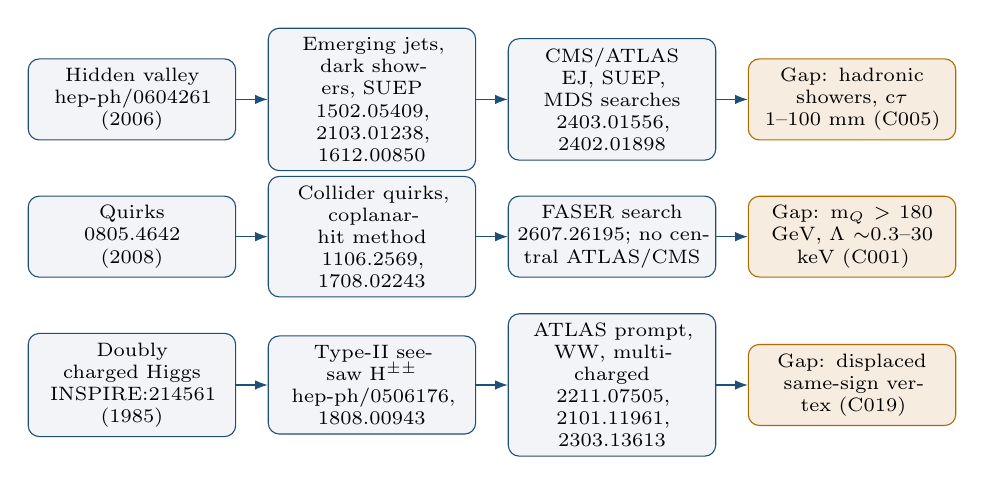
\begin{tikzpicture}[node distance=4mm,n/.style={draw=acc,rounded corners,fill=acc!6,font=\scriptsize,align=center,minimum height=0.9cm,text width=2.4cm},a/.style={-{Latex[length=1.6mm]},acc}]
\node[n](h){Hidden valley\\hep-ph/0604261\\(2006)};\node[n,right=of h](e){Emerging jets, dark showers, SUEP\\1502.05409, 2103.01238, 1612.00850};\node[n,right=of e](x){CMS/ATLAS EJ, SUEP, MDS searches\\2403.01556, 2402.01898};\node[n,right=of x,fill=warn!12,draw=warn](g){Gap: hadronic showers, c$\tau$ 1--100 mm (C005)};
\draw[a](h)--(e);\draw[a](e)--(x);\draw[a](x)--(g);
\node[n,below=7mm of h](k){Quirks\\0805.4642\\(2008)};\node[n,right=of k](k2){Collider quirks, coplanar-hit method\\1106.2569, 1708.02243};\node[n,right=of k2](k3){FASER search\\2607.26195; no central ATLAS/CMS};\node[n,right=of k3,fill=warn!12,draw=warn](k4){Gap: m$_Q>180$ GeV, $\Lambda\sim$0.3--30 keV (C001)};
\draw[a](k)--(k2);\draw[a](k2)--(k3);\draw[a](k3)--(k4);
\node[n,below=7mm of k](d){Doubly charged Higgs\\INSPIRE:214561\\(1985)};\node[n,right=of d](d2){Type-II seesaw H$^{\pm\pm}$\\hep-ph/0506176, 1808.00943};\node[n,right=of d2](d3){ATLAS prompt, WW, multi-charged\\2211.07505, 2101.11961, 2303.13613};\node[n,right=of d3,fill=warn!12,draw=warn](d4){Gap: displaced same-sign vertex (C019)};
\draw[a](d)--(d2);\draw[a](d2)--(d3);\draw[a](d3)--(d4);
\end{tikzpicture}\end{center}
The complete curated lineage for all 74 directions is in \texttt{research/literature/citation\_graph.md}; this is curated lineage, not an exhaustive citation network.
\section{Agents and models}
\subsection{Architecture}
The orchestrator (the main Claude Code session, Sonnet 5.5, medium effort) never read papers in depth. It held summaries, verdicts, logs, and wrote merge scripts. Sub-agents received a self-contained prompt, the shared rules file \texttt{methodology.md}, and a defined output location. The plan proposed Haiku for the cheapest steps; in practice \textbf{no Haiku agent was used}, because even the scouting stage required judgement about whether a gap sentence was real, so Sonnet was used for all cheap stages.
\subsection{Roles, models and counts}
\begin{center}\small\begin{tabular}{@{}p{3.3cm}p{1.5cm}r p{7.2cm}@{}}\toprule Role & Model & Runs & Task and independence rule\\\midrule
Literature scouts & Sonnet & 10 & One per topic cluster: top-cited and date-filtered searches, citation chains, gap phrases, PDF gap-sentence extraction; output candidate seeds and papers.\\
Gate 2 triage & Sonnet & 6 & Real coverage checks per merged direction (collaboration-filtered queries, public pages); PASS/HOLD/REJECT; reject only with a named covering result.\\
Gate 3 adversarial & Opus & 7 (+10 failed) & Try to kill each PASS direction; see only the neutral claim, not verdicts of other agents; DIES/NARROWED/SURVIVES.\\
Gate 4 experimental status & Opus & 5 + 3 reruns & ``Skeptical experimentalist'': exactly what is covered and what region is open.\\
Gate 4 feasibility & Opus & 5 + 3 reruns & Cross sections, yields, backgrounds, trigger, pileup, Phase-2 detector; HL-specific advantage.\\
Gate 4 theory deep-readers & Opus & 5 & Read source papers; assumptions, controlling parameters, robust vs model-dependent, constraints.\\
Arbiter & Strongest (fable) & 1 & Sees all four independent reports; scores, tiers, disagreement adjudication, citation audit, final documents.\\
\bottomrule\end{tabular}\end{center}
Totals: 16 Sonnet runs, 38 Opus runs launched (of which 20 were interrupted by session limits; their partial outputs were reused where saved), 1 arbiter run: \textbf{55 sub-agent launches}. Token use was not aggregated across agents.
\begin{caution}The user chose a ``lean'' budget of about 25 strong-model runs. Rate-limit failures and reruns meant 38 Opus runs were \emph{launched}, although 28 distinct Opus review tasks completed (7 adversarial, 8 experimental, 8 feasibility, 5 theory), some only after a rerun. This overrun should be borne in mind when planning stage~2.\end{caution}
\subsection{Independence and anti-bias rules}
\begin{itemize}
\item Gate 3 and Gate 4 reviewers were forbidden to read triage verdicts or other agents' outputs; they received the candidate's neutral claim and, at Gate~4, the proposed analysis target as a hypothesis to test.
\item Evidence rules shared by all agents: no unverifiable numbers, no ``new/first/unexplored'' as findings (a status taxonomy was used instead), ``not found'' is never proof of absence, every ID verified in INSPIRE.
\item The arbiter had to adjudicate disagreements explicitly and could not invent evidence.
\end{itemize}

\section{Results by stage}
\subsection{Funnel}
\begin{center}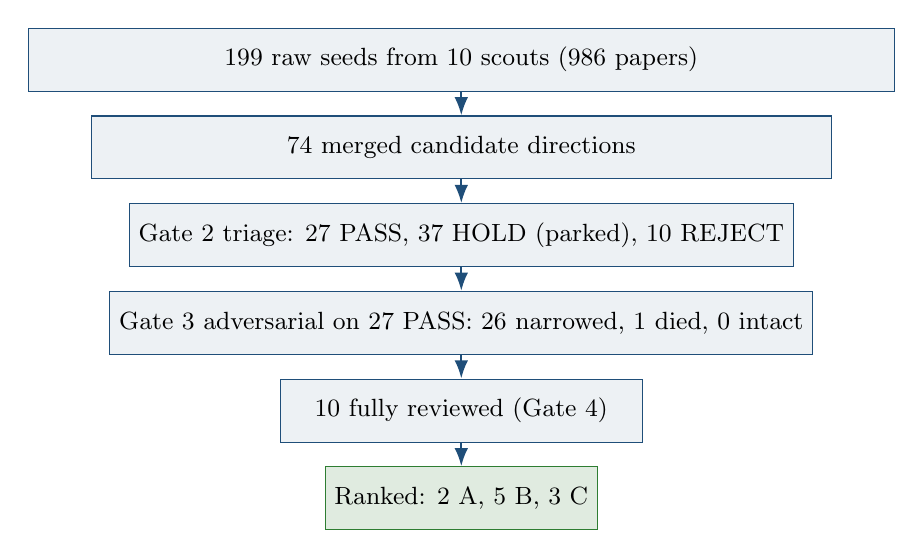
\begin{tikzpicture}[f/.style={draw=acc,fill=acc!8,align=center,font=\small,minimum height=0.8cm},arr/.style={-{Latex},acc,thick}]
\node[f,minimum width=11cm](a){199 raw seeds from 10 scouts (986 papers)};
\node[f,minimum width=9.4cm,below=3mm of a](b){74 merged candidate directions};
\node[f,minimum width=7.8cm,below=3mm of b](c){Gate 2 triage: 27 PASS, 37 HOLD (parked), 10 REJECT};
\node[f,minimum width=6.2cm,below=3mm of c](d){Gate 3 adversarial on 27 PASS: 26 narrowed, 1 died, 0 intact};
\node[f,minimum width=4.6cm,below=3mm of d](e){10 fully reviewed (Gate 4)};
\node[f,minimum width=3.2cm,below=3mm of e,fill=ok!15,draw=ok](g){Ranked: 2 A, 5 B, 3 C};
\foreach \x/\y in {a/b,b/c,c/d,d/e,e/g}{\draw[arr](\x)--(\y);}
\end{tikzpicture}\end{center}
\subsection{What the independent checks revealed}
The most important methodological result is that \textbf{scout headline gaps were frequently wrong}, because scouts judged coverage from titles and abstracts. Examples overturned at Gate~2/3:
\begin{itemize}
\item \textbf{$\sim$1\,cm lifetime blind spot} (``high confidence''): CMS 2409.10806 excludes B$>$1\% for c$\tau$ 1.5--370\,mm.
\item \textbf{RPV with displaced LSP}: ATLAS 2603.15007 reinterprets 13 searches across the coupling range.
\item \textbf{4D timing for LLPs (MTD/HGTD)}: the CMS MTD design report already projects displaced-vertex timing, delayed photons/jets and slow charged particles.
\item \textbf{Tau-philic leptoquark follow-up of the b-$\tau$ excess}: ATLAS 2503.19836 excludes the benchmark.
\item \textbf{A$\to$ZH in 2HDM}: CMS and ATLAS results plus an HL-LHC projection exist.
\end{itemize}
Even reviewers corrected each other: a misquoted ``5.7\,TeV'' leptoquark reach (actually the crossover with the atomic-parity-violation bound), an ATLAS result (2403.08547) that already excludes the photon-ISR benchmark in C008, and a branching-ratio claim for C015 that rests on a reviewer's own derivation and is kept only as a caveat.
\section{Ideas that survived: ranking}\label{sec:ranking}
The arbiter scored each of the ten fully reviewed candidates 0--5 on ten criteria (TI theoretical importance, PR phenomenological richness, EN experimental novelty, HL HL-LHC relevance, FE feasibility, SI potential sensitivity gain, SD signature distinctiveness, LG literature gap, TR theoretical robustness, PI publication impact). Experimental novelty and literature gap were capped at 2 when only a recast or projection remains. The ranking uses judgement and a veto rule first; the sum is shown but does not determine the order. \textbf{Tier A}: worth a dedicated analysis study. \textbf{B}: feasibility, recast or projection study first. \textbf{C}: insufficient or weak.
\begin{center}\scriptsize\setlength{\tabcolsep}{3.2pt}\begin{tabular}{rllrrrrrrrrrrrl}\toprule \# & ID & Tier & TI & PR & EN & HL & FE & SI & SD & LG & TR & PI & $\Sigma$ & Conf.\\\midrule
1 & C001 & A & 3 & 4 & 4 & 4 & 2 & 3 & 5 & 4 & 3 & 4 & 36 & Medium\\
2 & C005 & A & 3 & 4 & 3 & 4 & 3 & 3 & 3 & 3 & 3 & 3 & 32 & Medium\\
3 & C019 & B & 4 & 4 & 3 & 4 & 3 & 3 & 5 & 3 & 3 & 3 & 35 & Medium\\
4 & C044 & B & 4 & 4 & 2 & 4 & 4 & 3 & 4 & 2 & 3 & 3 & 33 & Medium\\
5 & C015 & B & 3 & 3 & 2 & 4 & 4 & 3 & 4 & 2 & 2 & 2 & 29 & Medium\\
6 & C051 & B & 3 & 3 & 3 & 3 & 4 & 2 & 3 & 3 & 3 & 3 & 30 & Medium\\
7 & C003 & B & 3 & 4 & 3 & 3 & 2 & 2 & 3 & 3 & 2 & 3 & 28 & Low\\
8 & C008 & C & 2 & 3 & 3 & 2 & 3 & 2 & 4 & 3 & 2 & 3 & 27 & Medium\\
9 & C040 & C & 3 & 2 & 2 & 4 & 3 & 2 & 2 & 2 & 3 & 2 & 25 & Medium\\
10 & C066 & C & 2 & 2 & 2 & 3 & 3 & 1 & 2 & 2 & 4 & 2 & 23 & Medium\\
\bottomrule\end{tabular}\end{center}
\subsection{Surviving gap for each candidate}
\subsubsection*{1. Quirks: coplanar non-helical tracks from EW-charged quirks (mesoscopic string regime) (tier A, Medium confidence)}
\textbf{Surviving gap.} Central-detector ATLAS/CMS search for coplanar, non-helical hit patterns from colour-neutral EW-charged quirks with m\_Q > $\sim$180 GeV and Lambda $\sim$0.3-30 keV (stated 0.1-100 keV is too wide: >30 keV gives a single straight HIP-like track; <$\sim$300 eV is covered by the HSCP recast).\\
\textbf{Status labels.} proposed-not-searched (ATLAS/CMS); LHC-not-projected-to-HL. \textbf{Kind:} experimental-analysis.\\
\textbf{Veto check.} No covering search: FASER 2607.26195 (forward, <=179 GeV at 10 keV) is the only LHC quirk search; HSCP/monojet recast 1703.00912 gives no bound for (1,1)\_-1 at 1 keV.
\\\textbf{Main feasibility obstacle} (feasibility reviewer, rating 2/5): Non-helical pattern recognition and trigger at PU 140-200 are undemonstrated; Z(nunu)+jets+PU coplanar background already $\sim$1e-2 fb at mu=50 (1911.02223) undermines the background-free premise; ISR-MET trigger eff $\sim$10\% for DY.

\subsubsection*{2. Higgs-portal dark showers with hadronic GeV dark mesons decaying in the tracker (multi-DV, VH/VBF tags) (tier A, Medium confidence)}
\textbf{Surviving gap.} Hadronic Higgs-portal dark showers with c*tau $\sim$1-100 mm (tracker) and m $\sim$5-20 GeV (natural core), in lepton-tagged VH (robust trigger) and, with a Phase-2 displaced L1 seed, ggF/VBF; multi-DV counting. CMS-side; ATLAS has a prospect study (INSPIRE 3201494).\\
\textbf{Status labels.} constrained-but-region-open; searched-limited-regime; LHC-not-projected-to-HL. \textbf{Kind:} experimental-analysis.\\
\textbf{Veto check.} Not vetoed: CMS MDS 2402.01898 covers Higgs-portal dark showers only at long c*tau (muon system, ggF); CMS 2409.10806 and ATLAS 2107.06092 cover the tracker region only for two-body H->SS (m\_a >= 16 GeV for ATLAS ZH). A recast of these could close part of the gap.
\\\textbf{Main feasibility obstacle} (feasibility reviewer, rating 3/5): Triggering ggF/VBF Higgs->soft displaced dark showers at PU200: Run-3 displaced-jet triggers keep only $\sim$0.4-1\% of H->SS, and the needed L1 displaced-track/vertex seed is not baseline. Second: low-mass (2-5 GeV) DV backgrounds (K\_S, material, B hadrons) prevent background-free counting.

\subsubsection*{3. Doubly charged scalars: displaced (charged-parent, same-sign) DVs; compressed cascades; hadronic taus (tier B, Medium confidence)}
\textbf{Surviving gap.} (i) Long-lived H++ (c*tau $\sim$0.1-100 mm) giving a charge-2 parent track ending in a same-sign/high-mass DV; TeV-scale only in the fermiophobic (GM-like) case, 100-150 GeV in neutrino-mass type-II. (iii) tau\_h H++ channels with full Run 2/3 and HL data. (ii) compressed soft same-sign leptons is systematics-limited ($\sim$1/5 feasibility).\\
\textbf{Status labels.} proposed-not-searched (displaced same-sign DV); indirectly-covered/not reinterpreted; searched-limited-regime (tau\_h); theory-explored-untested (compressed). \textbf{Kind:} experimental-analysis.\\
\textbf{Veto check.} Not vetoed, but a recast is required first: CMS 2110.04809 (displaced leptons, no charge or vertex requirement) and ATLAS 2410.16835 have partial acceptance that nobody has quantified; ATLAS 2601.05664 requires opposite charge.
\\\textbf{Main feasibility obstacle} (feasibility reviewer, rating 3/5): (i) Triggering on low-HT displaced W W decays plus the data-driven estimate of the fake high-mass DV tail at PU 200. Neither is demonstrated: the pheno assumes an ideal trigger and has inadequate background MC. (ii) An irreducible S/B of $\sim$3\% with unsimulated fakes.

\subsubsection*{4. VLQ exotic decays to new scalars: dedicated TT -> (tS0)(tS0) -> 6t; X5/3 -> t phi+ (W+ gamma) (tier B, Medium confidence)}
\textbf{Surviving gap.} A dedicated high-S\_T multilepton/multi-b search optimised for TT -> 6t above $\sim$1.6 TeV (recast already excludes 1.65 TeV at BR=1, 2609.00127), and an SSL + hard photon channel for X5/3 -> t W+ gamma (recast 1907.05894 says it is already constrained at the level of the standard channel).\\
\textbf{Status labels.} searched-limited-regime; indirectly-covered (recast to 1.65 TeV). \textbf{Kind:} experimental-analysis (optimisation of existing multilepton strategy).\\
\textbf{Veto check.} Not vetoed in mass reach above $\sim$1.6 TeV, but the region below is covered by recasts of SS2L/3L searches (2609.00127); diphoton S modes are directly covered (ATLAS 2607.28381, CMS 2610.03489); X5/3 -> tH+ covered (CMS-PAS-B2G-24-005).
\\\textbf{Main feasibility obstacle} (feasibility reviewer, rating 4/5): QCD pair-production cross section ceiling ($\sim$0.13 fb at 2 TeV, 14 TeV) combined with BR dilution in realistic models (effective BR(6t)$\sim$25\% for Br(T->tS)=50\%), against already-strong Run-2 limits (recast 6t: 1.65 TeV; CMS X5/3 1-lepton: 1.63-1.71 TeV) - the open window is $\sim$1.6-2.2 TeV with few events. For SSL+gamma: unknown jet->gamma / e->gamma fake...

\subsubsection*{5. Long-lived light ALPs from exotic top decays t -> q a (HCAL / muon system, lepton-triggered ttbar) (tier B, Medium confidence)}
\textbf{Surviving gap.} t -> q a with m\_a $\sim$1-35 GeV decaying in HCAL or muon system, presented model-independently as BR(t -> qX) vs (m\_X, c*tau). ATLAS 2403.15332 covers only m\_a = 40, 55 GeV in the ID.\\
\textbf{Status labels.} searched-limited-regime; constrained-but-region-open (as interpretation); LHC-not-projected-to-HL. \textbf{Kind:} experimental-analysis (signal reinterpretation / added signal regions).\\
\textbf{Veto check.} Partial coverage: ATLAS 2403.15332 directly covers m\_a 40-55 GeV (ID); ATLAS CalRatio+W 2407.09183 has a lepton-triggered selection that a t->qa event could pass but treats ttbar as background. Gap is largely an interpretation of existing analyses (rule 4).

\subsubsection*{6. High-mass Drell-Yan angular coefficients (A0-A2, T-odd A5-A7, l=3 harmonics) and sin2theta\_W running (tier B, Medium confidence)}
\textbf{Surviving gap.} Unfolded, phi-dependent A\_i above the Z peak vs m\_ll and pT\_ll, narrowed (theory reviewer) to the null tests A5-A7 and the l=3 basis of 2003.11615; A0-A2 off-peak only as a QCD test. Experimental MSbar sin2theta\_W(mu) extraction is PDF-limited and degenerate with contact interactions.\\
\textbf{Status labels.} one-observable-not-another; well-covered (high-mass A\_FB part). \textbf{Kind:} experimental-analysis (precision measurement).\\
\textbf{Veto check.} Partial veto: high-mass A\_FB and pT/y-integrated A0 already measured (CMS 2202.12327); that sub-idea is dead. Full A0-A7 only at the Z peak (CMS 2604.25678, ATLAS 1606.00689).
\\\textbf{Main feasibility obstacle} (feasibility reviewer, rating 3/5): Tiny event counts exactly where EFT effects grow (m\_ll>1.5 TeV, pT\_ll>100 GeV) combined with SM theory uncertainty on Lam-Tung violation and EFT degeneracies; for running: PDF uncertainty. Dim-6 dipoles already strongly bounded by other observables.

\subsubsection*{7. Displaced, hadronic, isotropic SUEP (plus an HL-LHC projection of the prompt SUEP programme) (tier B, Low confidence)}
\textbf{Surviving gap.} Isotropic soft displaced-track/vertex SUEP with c*tau $\sim$1 mm to a few cm from ggF/VH mediators; all SUEP searches use PV-associated tracks and prompt signals. Plus a collaboration HL-LHC projection of prompt SUEP.\\
\textbf{Status labels.} searched-limited-regime; constrained-but-region-open (displaced hadronic); LHC-not-projected-to-HL. \textbf{Kind:} experimental-analysis.\\
\textbf{Veto check.} Prompt SUEP well covered (CMS 2403.05311, 2607.09621, 2604.05996; ATLAS 2605.20015); displaced muonic covered (CMS 2511.11888); metre-scale by MDS. CMS states displaced SUEP 'would result in an emerging jet signature' (2403.05311).
\\\textbf{Main feasibility obstacle} (feasibility reviewer, rating 2/5): Displacement removes the primary-vertex association that is the only demonstrated SUEP-vs-QCD/pileup handle at PU200, while dark-meson products are too soft for the 2 GeV L1 track trigger: no viable trigger+background strategy shown for ggF; VH-lepton-tagged offline analysis is the only realistic path.

\subsubsection*{8. Photon-enriched semi-visible jets; photon-ISR-tagged low-mass Z' -> SVJ SVJ (tier C, Medium confidence)}
\textbf{Surviving gap.} (i) SVJ-gamma: high neutral-EM-fraction jets with non-isolated photons, vetoed by existing CMS SVJ selections (f\_gamma > 0.7 veto). (ii) photon-ISR low-mass SVJ survives only for B(Z'->chi chi) -> 1 and small g\_q.\\
\textbf{Status labels.} proposed-not-searched (SVJ-gamma); proposed-not-searched with partial indirect coverage (photon-ISR); LHC-not-projected-to-HL. \textbf{Kind:} experimental-analysis.\\
\textbf{Veto check.} (ii) benchmark of 2409.04741 (g\_q = 0.25) is excluded through its visible Z'->qq decays by ATLAS 2403.08547 (g\_q < 0.06-0.1 for 200-650 GeV). (i) not covered.
\\\textbf{Main feasibility obstacle} (feasibility reviewer, rating 3/5): (i) Instrumental high-NEMF fakes and calibration of photon-rich jets once the JetID NEMF cut is removed. (ii) Background modelling (gamma+jets and fake-photon multijet with fake MET) at low mass under PU200, with no worked limit even at Run-2 level.

\subsubsection*{9. Compressed direct stau pairs (stau-bino coannihilation corridor): collaboration HL-LHC projection (tier C, Medium confidence)}
\textbf{Surviving gap.} A collaboration-level Phase-2 projection for direct stau pairs with soft tau\_h + ISR/VBF + MET. Physics-motivated and reachable overlap is roughly Delta m $\sim$15-30 GeV, m(stau) $\sim$100-200 GeV.\\
\textbf{Status labels.} searched-limited-regime; LHC-not-projected-to-HL. \textbf{Kind:} experimental-analysis (projection only).\\
\textbf{Veto check.} Not vetoed in reach, but the analysis concept is already executed by ATLAS 2609.37215 (Run 2+3, ISR channel, no combined exclusion) and CMS 1910.01185; CMS review 2510.17971 says compressed-stau analyses are in preparation. Surviving gap is a projection (rule 4).
\\\textbf{Main feasibility obstacle} (feasibility reviewer, rating 3/5): Jet->tau\_h fake background at low tau pT under PU 140-200, with its systematic uncertainty. This saturates the gain from luminosity for dm < $\sim$20 GeV, where taus fall below $\sim$15-20 GeV ID thresholds. Second obstacle: the ISR/VBF requirement costs most of the small direct-stau cross section.

\subsubsection*{10. Resonant lepton-PDF single leptoquark with charm-tagged jets; collaboration HL projection (tier C, Medium confidence)}
\textbf{Surviving gap.} e/mu + c-tagged jet category in resonant lepton-quark fusion; in practice a flavour-rotation reinterpretation of the existing light-jet results plus a collaboration HL-LHC projection.\\
\textbf{Status labels.} one-observable-not-another; indirectly-covered; LHC-not-projected-to-HL. \textbf{Kind:} experimental-analysis (reinterpretation + projection).\\
\textbf{Veto check.} Indirectly covered: ATLAS 2507.03650 states u/c couplings are kinematically indistinguishable and reinterpretable by flavour rotation; CMS 2608.28377 states s/c sensitivity is bracketed by its u and b benchmarks. Third-generation sub-ideas (b tau, beta\_R, excess follow-up) die (ATLAS 2503.19836, CMS 2208.02717, 2308.06143, 2308.07826).
\\\textbf{Main feasibility obstacle} (feasibility reviewer, rating 3/5): c-quark x lepton PDF rate $\sim$28x below u at 2.5 TeV (2012.02092): matching u-reach needs y\_c >$\sim$3 (Gamma/M$\sim$0.2, broad, near perturbative edge); TeV-pT c-tagging low efficiency/poorly calibrated; and existing b-veto light-jet categories already accept c-jets (ATLAS 2507.03650 Sec.1 explicitly allows u/c reinterpretation), so incremental gain of c-tag category...

\begin{key}\textbf{Reading the ranking.} C001 ranks first because it is the clearest uncovered gap (no ATLAS/CMS central-detector quirk search was found), not because it is the easiest: its feasibility is the lowest of the ten. C044 has the most clearly HL-LHC-motivated case (background-free, statistics-limited) but the narrowest gap. Several candidates are essentially recasts or projections and the arbiter flagged them as such. The decision belongs to the physicist; \texttt{TOP\_CANDIDATES.md} contains the 12-section dossier for each.\end{key}

\section{Ideas that did not survive}
Rejections require a named covering result (or a physical showstopper); absence of a paper was never used as a reason. Gate~2 rejected \textbf{10} directions and Gate~3 one more.
\begin{center}\footnotesize\begin{tabular}{@{}l p{4.3cm} p{8cm}@{}}\toprule ID & Direction & Why rejected\\\midrule
C010 & Compressed / inelastic-DM soft displaced leptons and tracks & Positive evidence of broad coverage by 8+ CMS/ATLAS results over iDM, higgsino, VBF-compressed variants, plus HL-LHC projections. If re-raised, narrow to small-splitting (1-5\%) iDM.\\
C020 & Electroweak-charged dark mesons (5-plet) & Model-specific interpretation of existing signatures (authors recast them themselves); no new observable. Not a literal experimental result for the model, hence status indirectly-covered.\\
C024 & Top/gluon-philic ALP and heavy (pseudo)scalar tt... & Positive evidence of experiment-level interference-aware search over 365-1000 GeV; remaining radion-specific details are interpretation only.\\
C028 & $\sim$1 cm lifetime blind spot (H->phi phi->4j, L1 track trigger) & Positive evidence that CMS 2409.10806 covers c*tau $\sim$1 cm for H->SS->4b/4d with ggF triggers, with limits stated in conclusions.\\
C033 & Main-detector vs far-detector complementarity (GeV LLPs) & Fails Q1: a detector-comparison framing, not a collider observable CMS/ATLAS can measure; GeV-scale LLP main-detector coverage exists (2409.10806, 2403.15332, 2606.25840). Fold into C027.\\
C034 & R-hadrons, gluinonium, mini-split displaced/stopped... & Charge-flip and stopped R-hadron modelling already treated in CMS 2410.09164 and ATLAS 2104.03050/2502.06694; remaining gluinonium piece not supported by evidence of HL-LHC reach.\\
C035 & RPV with intermediate-lifetime displaced LSP & Broad framing is directly covered by ATLAS 2603.15007 (+CMS DV/displaced-lepton searches); no specific uncovered signature remains in this candidate.\\
C067 & Mixed-decay third-gen LQ (b nu t tau) & Scout seed's premise ('no search for the mixed b nu t tau final state') is contradicted by CMS 2012.04178 which names this exact signature. S3/mixed t-mu / b-nu cases are covered by ATLAS 2401.11928 and CMS...\\
C070 & Charm- and strange-flavoured leptoquarks & Scout statement 'ATLAS has a c-tag + MET search; l+c-tag resonance not seen' is true only for single/resonant; pair-production l+c-tag is in ATLAS 2006.05872 and LQ->c nu in ATLAS 2410.17824. Remaining gap is...\\
C073 & Unparticles / mass-gapped conformal sector & Positive evidence of CMS unparticle interpretations (1408.3583, 1701.02042, r925365) and hidden-valley coverage; no distinct observable left; theory interest low (no post-2019 INSPIRE hits). Caveat: Run 2...\\
C026 (G3) & 4D (space+time) displaced vertices and timing for... & Only a marginal residual survives: (i) ATLAS HGTD (2.4<|eta|<4) timing for forward LLP decay products, since the ATLAS HGTD TDR contains no LLP timing study; physics value is limited because forward tracker...\\
\bottomrule\end{tabular}\end{center}
In addition, 24 HOLD directions were \emph{parked} (not rejected): promising but without a review budget. Five alternates were identified for a possible extra pass: C017 (pseudo-Dirac heavy neutrinos, time-resolved lepton-number-violation oscillations), C061 (HHH beyond 6b), C009 (semi-dark Higgs decays), C047 (portal-matter vector-like quarks to dark photons) and C048 (colour-sextet top partners).
\section{Problems encountered and lessons}
\begin{enumerate}
\item \textbf{Session rate limits.} Gate~3 failed once with no saved output; Gate~4 failed for all ten first-wave agents. After the first failure all agents were told to save incrementally; after the second, 14 of 20 Gate~4 reviews were already on disk and only six were rerun. \emph{Lesson:} require per-candidate saving and stagger large opus fan-outs.
\item \textbf{Cost overrun relative to the lean budget:} 38 Opus launches versus the planned $\sim$25, a direct consequence of the failures above.
\item \textbf{Weak first-pass coverage claims.} Scouts and parts of the triage used title/abstract-level queries; ``no CMS/ATLAS search found'' proved unreliable. The adversarial and experimental reviews, which read the closest results, repeatedly overturned scout conclusions.
\item \textbf{Subagent spawning.} In the first Gate~3 attempt, batch agents spawned extra per-candidate agents (3 extra failed Opus launches); later prompts forbade it.
\item \textbf{Shared-scratch collisions.} Several scouts overwrote each other's temporary files. One scout's early query log was reconstructed from memory (papers and quotes unaffected).
\item \textbf{Duplicate completion notices} from some scouts (leftover monitors) cluttered the log but changed no results.
\item \textbf{Tool quirks.} INSPIRE \texttt{abstract "..."} returns nothing (use \texttt{abstracts.value:}); \texttt{refersto:arxiv:} returns junk (use recid); WebFetch is lossy, so stau cross sections taken from a web page need re-checking; two-column PDFs garble extracted gap quotes (flagged, re-verified before citing).
\item \textbf{Stale gap statements.} Some ``future work'' quotes came from old documents (e.g.\ a 2018 MATHUSLA white paper) and had been overtaken by later work.
\item \textbf{Reviewer disagreements} resolved by the arbiter: C040 mass-splitting window (theory $\lesssim$30\,GeV vs feasibility $\gtrsim$15\,GeV), C066 ``5.7\,TeV'' misquote, C008 photon-ISR exclusion, C015 coupling caveat, C019 coverage by CMS 2110.04809 (no charge requirement).
\end{enumerate}
\section{Limitations}
\begin{itemize}
\item Coverage of the literature is broad but not exhaustive; INSPIRE title/abstract queries miss full-text mentions and some CMS PAS / ATLAS-CONF notes.
\item Only 10 of 74 directions received full independent review; the rest are triage-level.
\item Small calculations in the feasibility reviews are back-of-envelope estimates, labelled as such; no sensitivity projections were produced.
\item Sonnet-level triage and scouting may contain errors that were not revisited for parked directions.
\item Two numbers are \textsc{unverified}: a CMS $\tau\tau$ H$^{\pm\pm}$ limit quoted as both 535 and 396\,GeV in different sources, and the content of CMS-PAS-B2G-24-005 (read at abstract level only).
\end{itemize}
\section{Status and next steps}
The workflow has reached the \textbf{human checkpoint}. Options:
\begin{enumerate}
\item Choose one candidate (or a combination) for stage~2: strategy, literature, sample exploration, selection, backgrounds and systematics, with an independent review at each phase.
\item Spend more review budget on the parked directions or the five alternates.
\item Ask for deeper checks on a particular candidate (e.g.\ a recast of CMS 2110.04809 for C019 before treating it as open).
\end{enumerate}
\section*{Appendix: workspace map}
\begin{small}\begin{tabular}{@{}p{5.2cm}p{9.5cm}@{}}\toprule Path & Content\\\midrule
\texttt{RESEARCH\_PLAN.md} & plan: architecture, strategy, scoring, gates, stopping criteria\\
\texttt{TOP\_CANDIDATES.md} & 12-section dossier for the 10 reviewed candidates, lineage, how to choose\\
\texttt{REJECTED\_CANDIDATES.md} & rejected directions, killed sub-ideas, overturned scout claims\\
\texttt{research/literature/} & scout outputs, \texttt{papers.json}, \texttt{seminal\_papers.md}, \texttt{citation\_graph.md}\\
\texttt{research/candidates/} & raw seeds, merged directions, gate verdicts, candidate database\\
\texttt{research/reviews/} & triage, adversarial, experimental, feasibility, theory reviews\\
\texttt{research/rankings/, reports/} & ranking, literature review, citation audit\\
\texttt{research/LOG.md} & chronological log including failures\\
\texttt{research/tools/} & helper scripts (INSPIRE, PDF, merge, report generation)\\
\bottomrule\end{tabular}\end{small}
\end{document}
